\section{Results}
%
\subsection{ADC Setup and dead time}
%
We digitize and record our data with an \textbf{Analog to Digital Converter} (ADC).
Such a device always has a finite dead time $\tau$ after detecting an incoming signal.
If another signal follows in that time it will not be registered.
This changes the accepted detection rate $R_{\text{acc}}$ compared to the actual rate $R_{\text{in}}$.
Over a time corresponding to $\tau \cdot R_{\text{acc}}$ we do not record any additional photons.
The rate of additional incoming photons in that time can be calculated by multiplying with $R_{\text{in}}$.
We get:
\begin{align}
    \label{eq:DeadTime}
    \begin{split}
        R_{\text{in}} &= R_{\text{acc}} \cdot (1 + \tau \cdot R_{\text{in}} )
    \end{split}
\end{align}
%
\subsection{Energy calibration}
%
Using the recorded spectra, we can determine a functional relation between channel and energy.
We plot the channel number $\xi$ of the distinct photo peaks against the theoretic energy value $E$ taken from \cite{Anleitung}.
The result is shown in figure \ref{fig:EnergyCalibration}.
As an error we use the FWHM of the peak.
With the \texttt{scipy.curvefit} Python function we fit an affine linear function to the data.
%
\par
%
\minipage{\linewidth}
    \begin{center}
        \captionsetup{type=figure}
        \begin{adjustbox}{max width=\linewidth, keepaspectratio}
            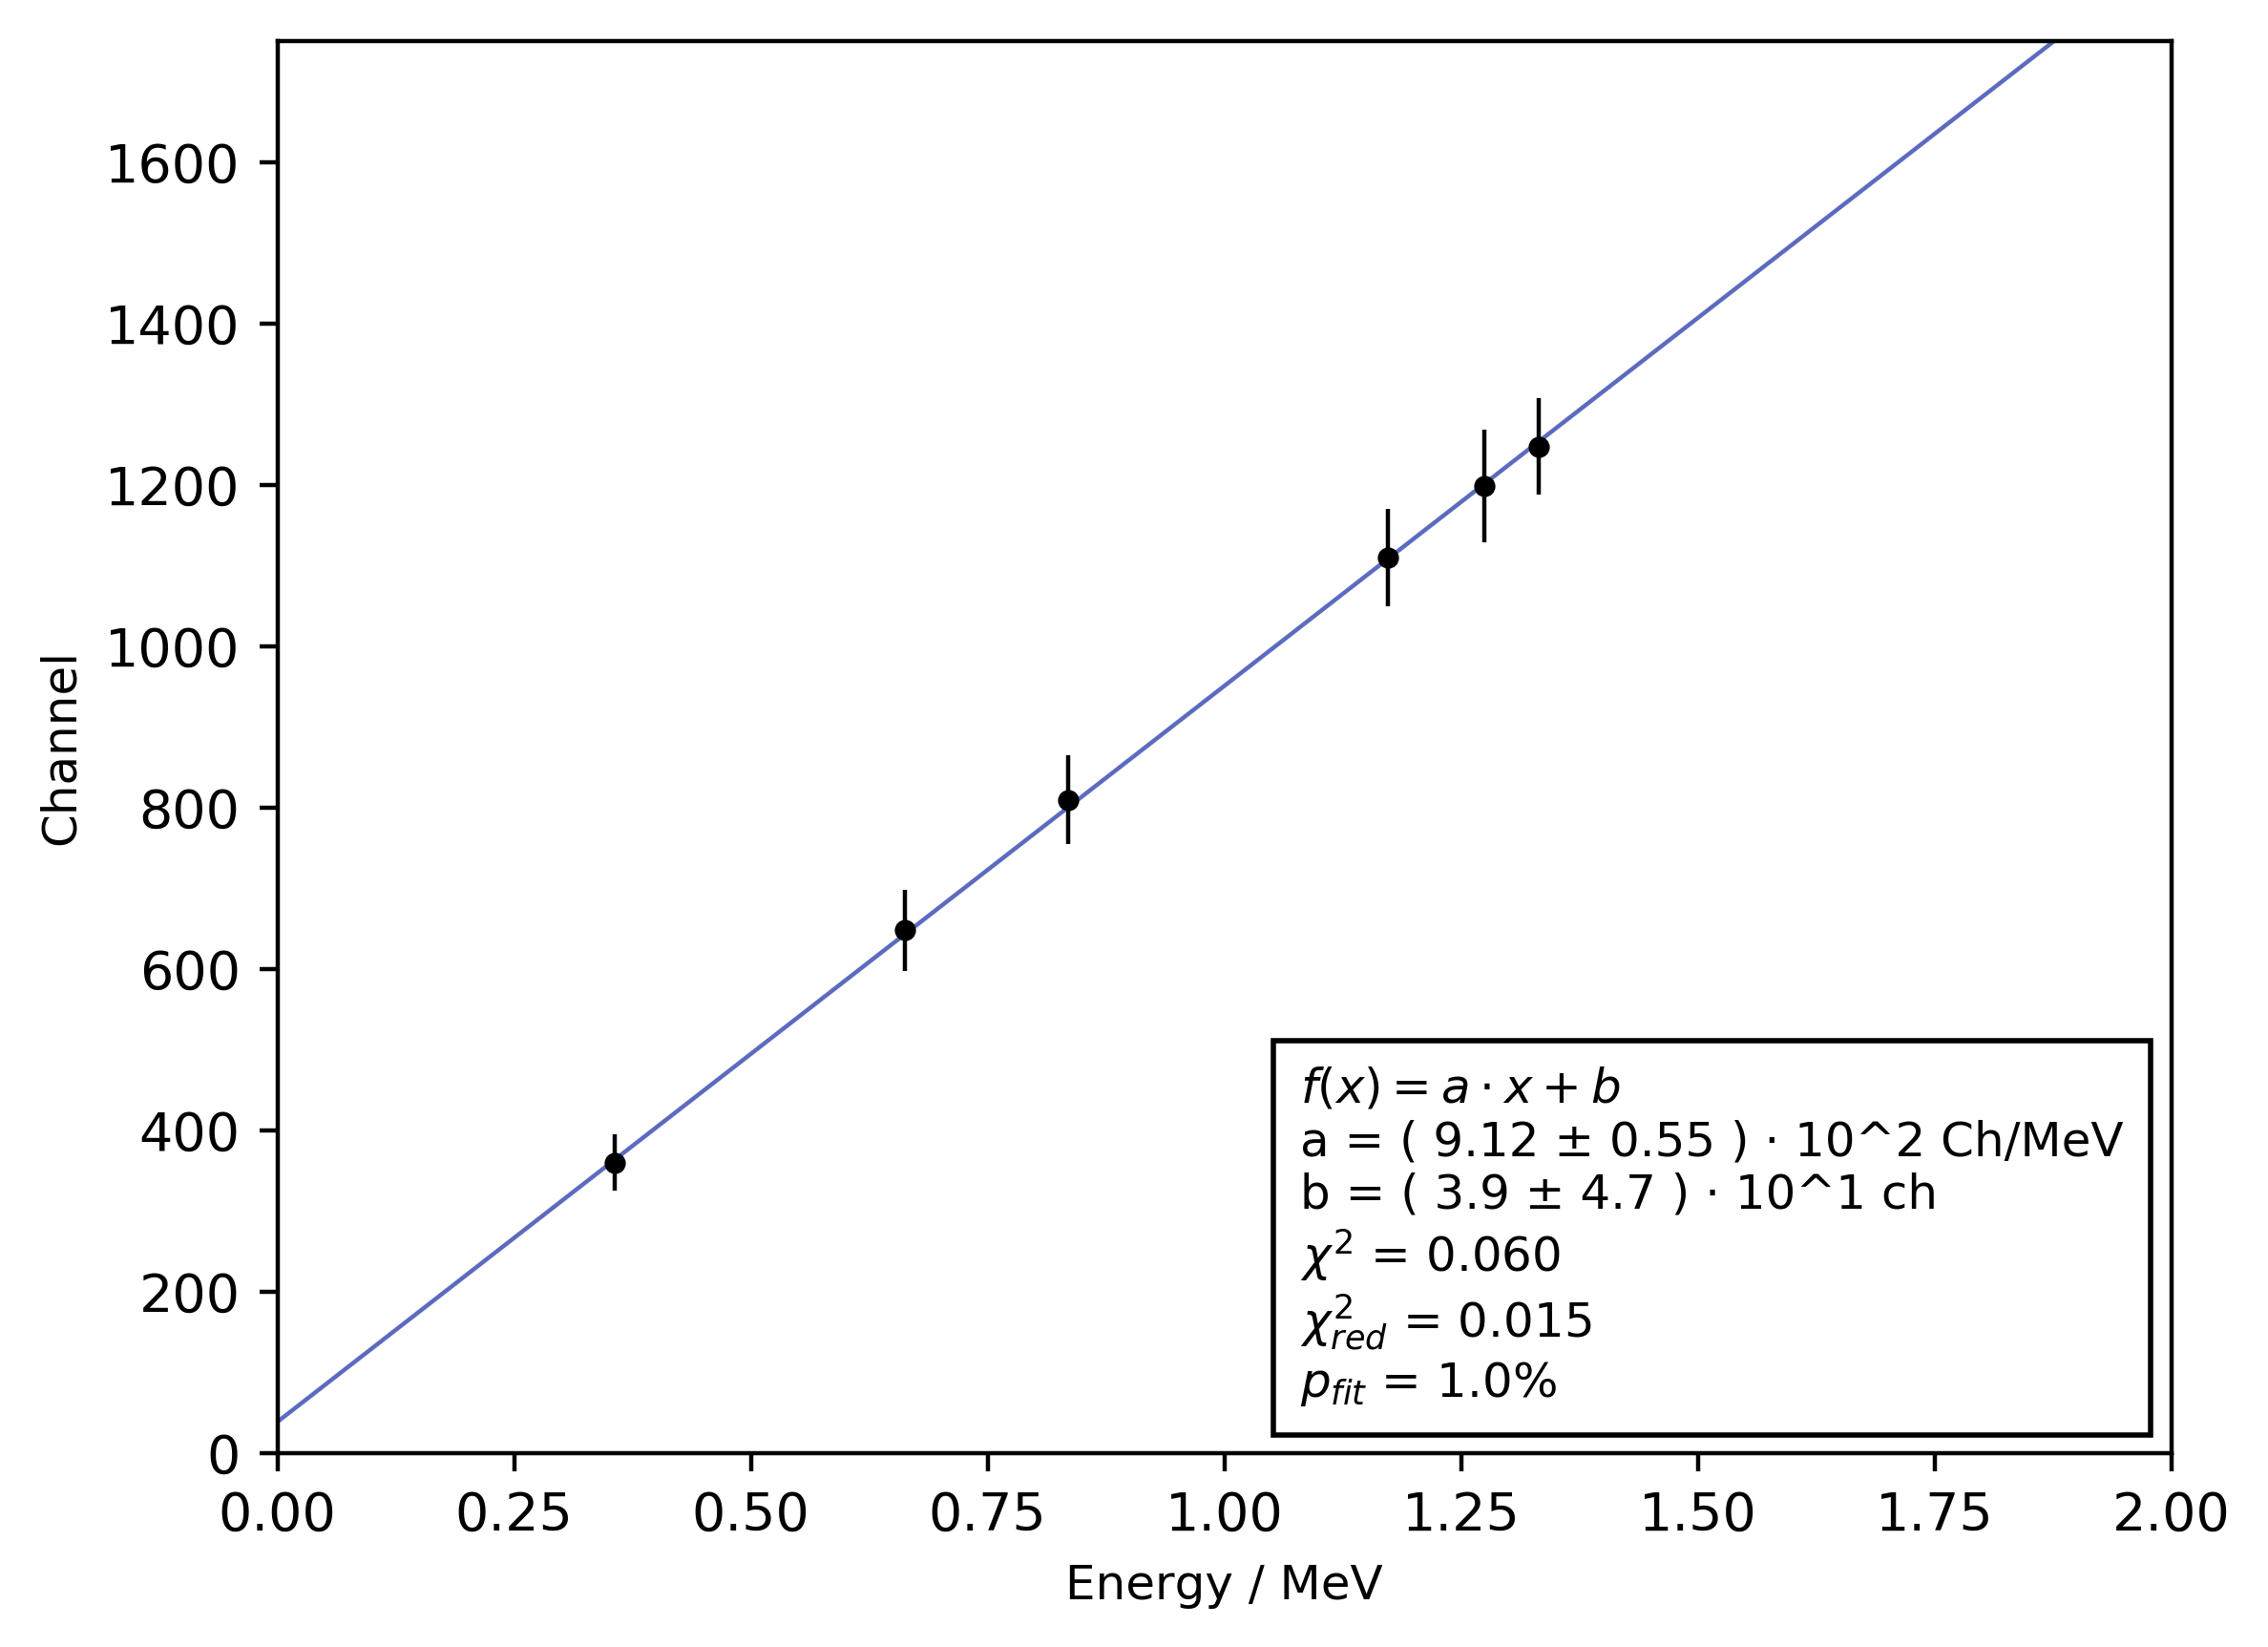
\includegraphics[]{png/energy_calibration}
        \end{adjustbox}
        \captionof{figure}{Energy calibration}
        \label{fig:EnergyCalibration}
    \end{center}
\endminipage
%
\par
%
From the fit parameters (see figure \ref{fig:EnergyCalibration}) we can now calculate the energy corresponding to any channel $\xi$:
\begin{align}
    \label{eq:}
    \begin{split}
        E &= \frac{\xi - b}{a}
    \end{split}
    \\
    \label{eq:}
    \begin{split}
        \Delta E &= \sqrt{ \left ( \frac{ \Delta a}{ a } \right ) ^2 + \left ( \frac{\Delta b}{b} \right ) ^2 } \cdot E
    \end{split}
\end{align}
%
\subsection{Energy resolution}
%
The energy $E$ registered by our computer is proportional to the number of photons $N$ coming from the photo multiplier:
\begin{align}
    \label{eq:}
    \begin{split}
        E \sim N \implies \Delta E \sim \Delta N = \sqrt{N}
    \end{split}
    \\
    \label{eq:}
    \begin{split}
        \implies \frac{\Delta E}{E} \sim \frac{1}{\sqrt{N}} \sim \frac{1}{\sqrt{E}}
    \end{split}
\end{align}
%
In figure \ref{fig:EnergyResolution} we plot the relative error $\frac{\Delta E}{E}$ of all marked features against the energy $E$ to see this relation.
For $\Delta E$ we use the FWHM of the peak at the corresponding channel $\xi$.
To calculate the FWHM, we effectively use the difference between two channels.
With value $b$ from the energy calibration we get in total:
\begin{align}
    \label{eq:}
    \begin{split}
        \frac{\Delta E}{E} &= \frac{ \Delta \xi }{\xi - b}
    \end{split}
    \\
    \label{eq:}
    \begin{split}
        \Delta \left ( \frac{\Delta E}{E} \right ) &= \frac{ \Delta b }{ b } \cdot \frac{\Delta E}{E}
    \end{split}
\end{align}
%
To these data points we fit the above described relation $f(x) = \frac{A}{\sqrt{x}} + B$ and obtain the fit parameters as seen in figure \ref{fig:EnergyResolution}.
Here, $B$ is an additional bias term not motivated by physics but to account for systematic errors.
%
\par
%
\minipage{\linewidth}
    \begin{center}
        \captionsetup{type=figure}
        \begin{adjustbox}{max width=\linewidth, keepaspectratio}
            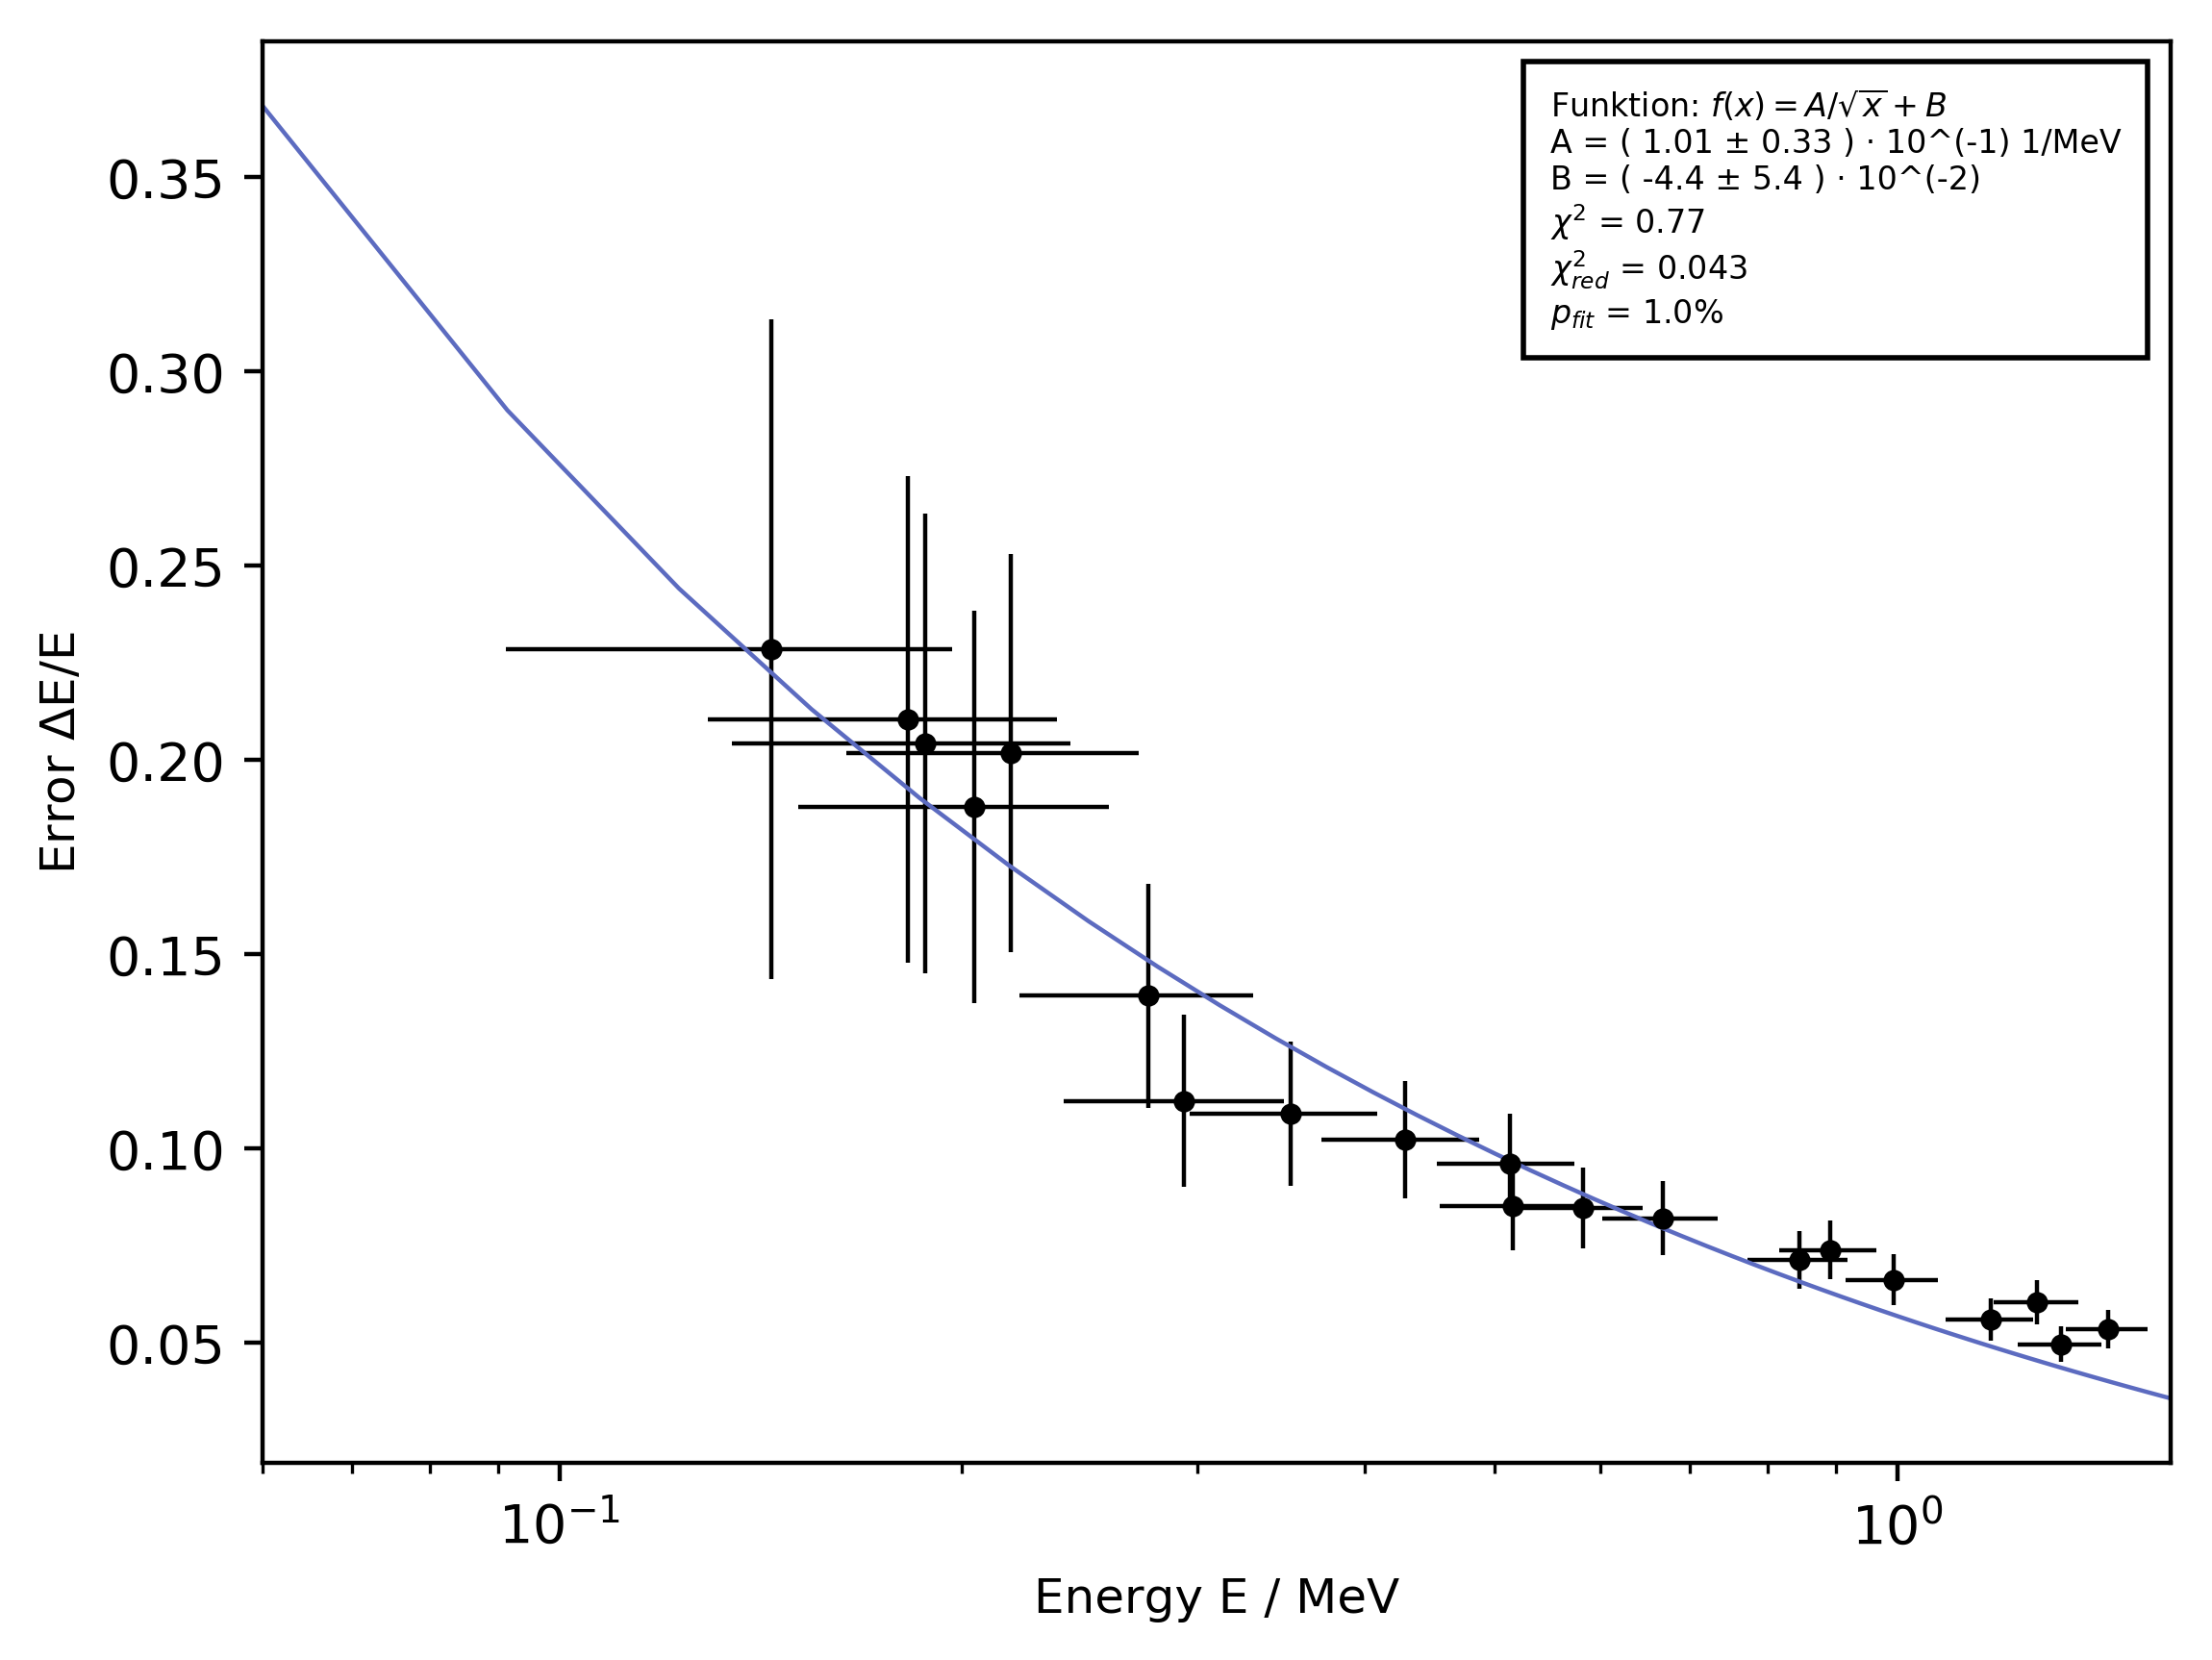
\includegraphics[]{png/energy_resolution}
        \end{adjustbox}
        \captionof{figure}{Energy resolution}
        \label{fig:EnergyResolution}
    \end{center}
\endminipage
%
\subsection{Spectra of different radioactive nuclei}
%
To analyze our recorded spectra we take a look at the distinct peaks and edges.
In table \ref{tab:EnergyComparison} we compare the experimentally measured and the theoretic energies for all spectra quantitatively.
The theoretical values are taken from \cite{Anleitung} if not stated otherwise.
Below, we give a physical explanation for the most prominent features of each spectrum.
The sharp cutoff below channel $\xi = 130$ is most likely due to software configuration as it is observable in all spectra.
%
\par
%
\minipage{\linewidth}
    \begin{center}
        \captionsetup{type=table}
        \begin{adjustbox}{max width=\linewidth, keepaspectratio}
            \begin{tabular}{lllll}
            \toprule
            Sample            & Type             & $E_{\text{exp}}$ [\SI{}{\mega\electronvolt}] & $E_{\text{theo}}$ [\SI{}{\mega\electronvolt}] & Deviation      \\
            \midrule
            $^{60}\text{Co}$  & backscatter peak & 0.22 $\pm$ 0.04                              & 0.21                                          & 0.17  $\sigma$ \\
            ~                 & Compton edge     & 0.89 $\pm$ 0.07                              & 0.96                                          & 1.1   $\sigma$ \\
            ~                 & photo peak       & 1.17 $\pm$ 0.07                              & 1.17                                          & 0.014 $\sigma$ \\
            ~                 & photo peak       & 1.33 $\pm$ 0.07                              & 1.33                                          & 0.11  $\sigma$ \\
            $^{137}\text{Cs}$ & backscatter peak & 0.19 $\pm$ 0.04                              & 0.18                                          & 0.090 $\sigma$ \\
            ~                 & Compton edge     & 0.43 $\pm$ 0.04                              & 0.48                                          & 1.1   $\sigma$ \\
            ~                 & photo peak       & 0.67 $\pm$ 0.05                              & 0.66                                          & 0.11  $\sigma$ \\
            $^{54}\text{Mn}$  & backscatter peak & 0.20 $\pm$ 0.04                              & 0.20                                          & 0.22  $\sigma$ \\
            ~                 & Compton edge     & 0.58 $\pm$ 0.05                              & 0.64                                          & 1.2   $\sigma$ \\
            ~                 & photo peak       & 0.85 $\pm$ 0.06                              & 0.84                                          & 0.17  $\sigma$ \\
            $^{133}\text{Ba}$ & backscatter peak & 0.14 $\pm$ 0.03                              & 0.16                                          & 0.52  $\sigma$ \\
            ~                 & Compton edge     & 0.29 $\pm$ 0.03                              & 0.28                                          & 0.52  $\sigma$ \\
            ~                 & photo peak       & 0.35 $\pm$ 0.04                              & 0.36                                          & 0.10  $\sigma$ \\
            $^{22}\text{Na}$  & backscatter peak & 0.18 $\pm$ 0.04                              & 0.17                                          & 0.31  $\sigma$ \\
            ~                 & Compton edge     & 0.28 $\pm$ 0.04                              & 0.34                                          & 1.7   $\sigma$ \\
            ~                 & photo peak       & 0.52 $\pm$ 0.04                              & 0.51                                          & 0.10  $\sigma$ \\
            ~                 & Compton edge     & 0.99 $\pm$ 0.07                              & 1.06                                          & 1.04  $\sigma$ \\
            ~                 & photo peak       & 1.27 $\pm$ 0.08                              & 1.27                                          & 0.037 $\sigma$ \\
            Night             & -                & 0.51 $\pm$ 0.05                              & 0.51                                          & 0.056 $\sigma$ \\
            ~                 & -                & 1.44 $\pm$ 0.08                              & 1.31                                          & 1.6   $\sigma$ \\
            \bottomrule
            \end{tabular}
        \end{adjustbox}
        \captionof{table}{Comparison of experimental and theoretical energies of relevant processes. The deviation is calculated before rounding the results.}
        \label{tab:EnergyComparison}
    \end{center}
\endminipage
%
\subsubsection{Spectrum of $^{60}\text{Co}$}
%
In 99\% of all cases \textbf{$^{60}\text{Co}$} decays in a $\beta^{+}$ decay into an exited state of $^{60}\text{Ni}$, which in turn emits its energy in two stages as seen in figure \ref{fig:60CoDecayScheme}.
The corresponding photons cause the two most intense peaks.
Their energies do not deviate significantly from the theoretically expected values.
The spectrum also shows the characteristic Compton continuum with an edge visible at roughly \SI{0.89}{\mega\electronvolt}.
The measurement corresponds to the theoretical edge for the lower energy disexcitation.
Since the two values overlap, the edge is not very sharp and also lies within the general region of the second expected value.
At \SI{0.217}{\mega\electronvolt}, we see one peak of backscattered photons resulting from the Compton effect.
Here, the theoretical peaks overlap a lot and the measured data fits both of them.
%
\subsubsection{Spectrum of $^{137}\text{Cs}$}
%
\textbf{$^{137}\text{Cs}$} decays trough $\beta^{+}$ into an exited $^{137}\text{Ba}$, which is a metastable state with a \SI{2.55}{\minute} life span caused by the forbidden high polarity transmission \mbox{$\nicefrac{11}{2}^{-} \rightarrow \nicefrac{3}{2}^{+}$} as seen in figure \ref{fig:137CsDecayScheme}.
Eventually it decays by photon emission (90\%) resulting an the peak at \SI{0.668}{\mega\electronvolt} or internal conversion (10\%), where the nucleus transfers energy electromagnetically to a shell electron.
This not only results in the detection of electrons of different energy after ionization, but also yields additional coincident photons emitted when the ion absorbs a free electron.
These effects smear out spectrum a bit, but we still see the relevant peaks.
Again we also see the Compton edge and backscatter peak of the main photon at their expected positions.
%
\subsubsection{Spectrum of $^{54}\text{Mn}$}
%
\textbf{$^{54}\text{Mn}$} decays by electron capture leading to an exited state of $^{54}\text{Cr}$ (see figure \ref{fig:54MnDecayScheme}).
The resulting photons create the visible peak with matching energy.
We also get the expected Compton edge and backscatter peak.
%
\subsubsection{Spectrum of $^{133}\text{Ba}$}
%
\textbf{$^{133}\text{Ba}$} decays through electron capture into two different exited states of $^{133}\text{Cs}$.
As can be seen in figure \ref{fig:133BaDecayScheme}, the decay scheme allows many possible electron transitions enabling a multitude of different peaks in the spectrum.
Many of these however are either rather unlikely (high polarity transmission) or overlap.
Quantitatively we can only examine three pronounced peaks (see table \ref{tab:EnergyComparison}).
The highest energy one matches the energy of the \mbox{$\nicefrac{1}{2}^{+} \rightarrow \nicefrac{5}{2}^{+}$} transmission with 91\% probability.
Since it is the most likely transmission it also shows the highest peak.
The second peak presumably belongs to the \mbox{$\nicefrac{3}{2}^{+} \rightarrow \nicefrac{5}{2}^{+}$} transmission (65\%), the energy here also corresponds within its margin of error.
The lowest peak is very wide but could be caused by the \mbox{$\nicefrac{5}{2}^{+} \rightarrow \nicefrac{7}{2}^{+}$} transmission (12\%).
The energies do not differ significantly.
At this energy we also expect the Compton continuum and backscatter peaks, explaining the width of the peak.
At around \SI{0.062}{\mega\electronvolt} (channel 95) we can see a very faint peak, which could correspond to the \mbox{$\nicefrac{5}{2}^{+} \rightarrow \nicefrac{5}{2}^{+}$} transmission with 88\% probability.
However the position and error can not be estimates due to the low count number.
Here we could have used a higher coarse gain at the amplifier.
%
\par
%
We can not quantitatively observe any of the coincident events, since they are either unlikely or of too low energy for us to register.
The electron for the electron capture is taken from the electron shell.
Therefore, after the decay, the daughter nucleus is in an ionized state.
During the following neutralization there is a photon emitted, with a characteristic energy depending on the energy level of the captured electron.
For the $^{133}\text{Cs}$ radionuclide we find binding energies of around \SI{36}{\kilo\electronvolt}. \cite{KayeLaby}
These are too low for us to detect with our setup.
%
\subsubsection{Spectrum of $^{22}\text{Na}$}
%
\textbf{$^{22}\text{Na}$} decays mostly in $\beta^{+}$ and electron capture into an exited state of $^{22}\text{Ne}$ which then loses its energy after \SI{3}{\pico\second} in a simple dipole transmission.
This energy matches the one of out high energy peak at \SI{1.272}{\mega\electronvolt}.
These photons can also lose their energy in the Compton effect creating the slightly visible Compton edge at channel 945, matching the theoretical value.
The intense peak at channel 509 is caused by the $\beta^{+}$ decay.
The created positrons are slowed down and annihilate with surrounding electrons.
Due to spin conservation this yields two photons with one electron resting energy (\SI{511}{\kilo\electronvolt}) each.
At low energies we see the Compton edge and backscatter peak of the annihilation photons.
Their energies match the theoretical values.
As one would expect, because of the high intensity of the annihilation peak the backscatter peak of the high energy photons is predominated and not separately visible.
%
\subsubsection{Night measurement}
%
In the \textbf{night measurement} we can observe two clear peaks.
The high energy one matches the value for the $^{40}\text{K}$ $\beta^{-}$ decay (90\%) \cite{WikiPotassium}.
Potassium is a naturally occurring element on earth and about 0,0117\% is of the radioactive isotope $^{40}\text{K}$.
The second peak lies very close to the electron resting energy.
This leads to the suspicion, that it is caused by electron annihilation as in $^{22}\text{Na}$.
However $\beta^{+}$ decay of $^{40}\text{K}$ is actually quite unlikely (0,001\%) \cite{WikiPotassium}, so other explanations may be more likely.
For lower energies we see an increase in the spectrum.
This is the expected result for bosonic particles, lower energies are more probable.
%
\subsection{Coincidence measurement of $^{137}\text{Cs}$}
%
\subsubsection{Simple coincidence spectrum}
%
As before, the spectrum seen in figure \ref{fig:137Cskoinz1} shows the three peaks at their expected theoretical positions.
However, because the Linear Gate only allows detection on counter 1 when there is also a signal registered at counter 2.
Therefore, the photo peak is reduced in intensity because it is only registered due to random coincidence.
The Compton edge and backscatter peak in contrast occur coincidentally and are more prominent.
By using the Delay Amplifier with a time $t_{\text{delay}}$, we made sure that signal 1 coming in at $t_1$ entered the Linear Gate after signal 2 at tine $t_2$ went trough the TSCA and opened the Linear Gate.
If the latter is then open for a time of $t_{\text{trigger}}$, we get the following constraint for the respective times: $t_2 < t_1 + t_{\text{trigger}} < t_2 +  t_{\text{delay}}$.
The coincidence resolution is then given directly by $t_{\text{trigger}}$.
%
\subsubsection{Random coincidence}
%
If we deliberately increase $t_{\text{delay}}$, the two coincident events of Compton edge and backscatter peak will never arise at the same time.
This results in figure \ref{fig:137Cskoinz2} where only the photo peak is visible, because random coincidence still occurs as before.
%
\subsubsection{Improved method}
%
The time spectra in figures \ref{fig:137CsTPHC}, \ref{fig:137CsTPHC20ns}, \ref{fig:137CsTPHC40ns} and \ref{fig:137CsTPHC60ns} all show a single peak which corresponds to the time between the detection of a Compton-scattered electron in one detector and the corresponding photon in the other.
The noise level is caused by random coincidence which happened with no particular time difference.
The added delay only shifts the peak along the channel axis.
This relation between channel time allows us to calculate the time calibration of the circuit.
In figures \ref{fig:TimeCalibrationCs} and \ref{fig:TimeCalibrationCo} we plot the peak channels of the differently delayed spectra against the delay time.
We fit a linear function to the points to get the channel-energy relation $a$.
%
\par
%
\minipage{\linewidth}
    \begin{center}
        \captionsetup{type=figure}
        \begin{adjustbox}{max width=\linewidth, keepaspectratio}
            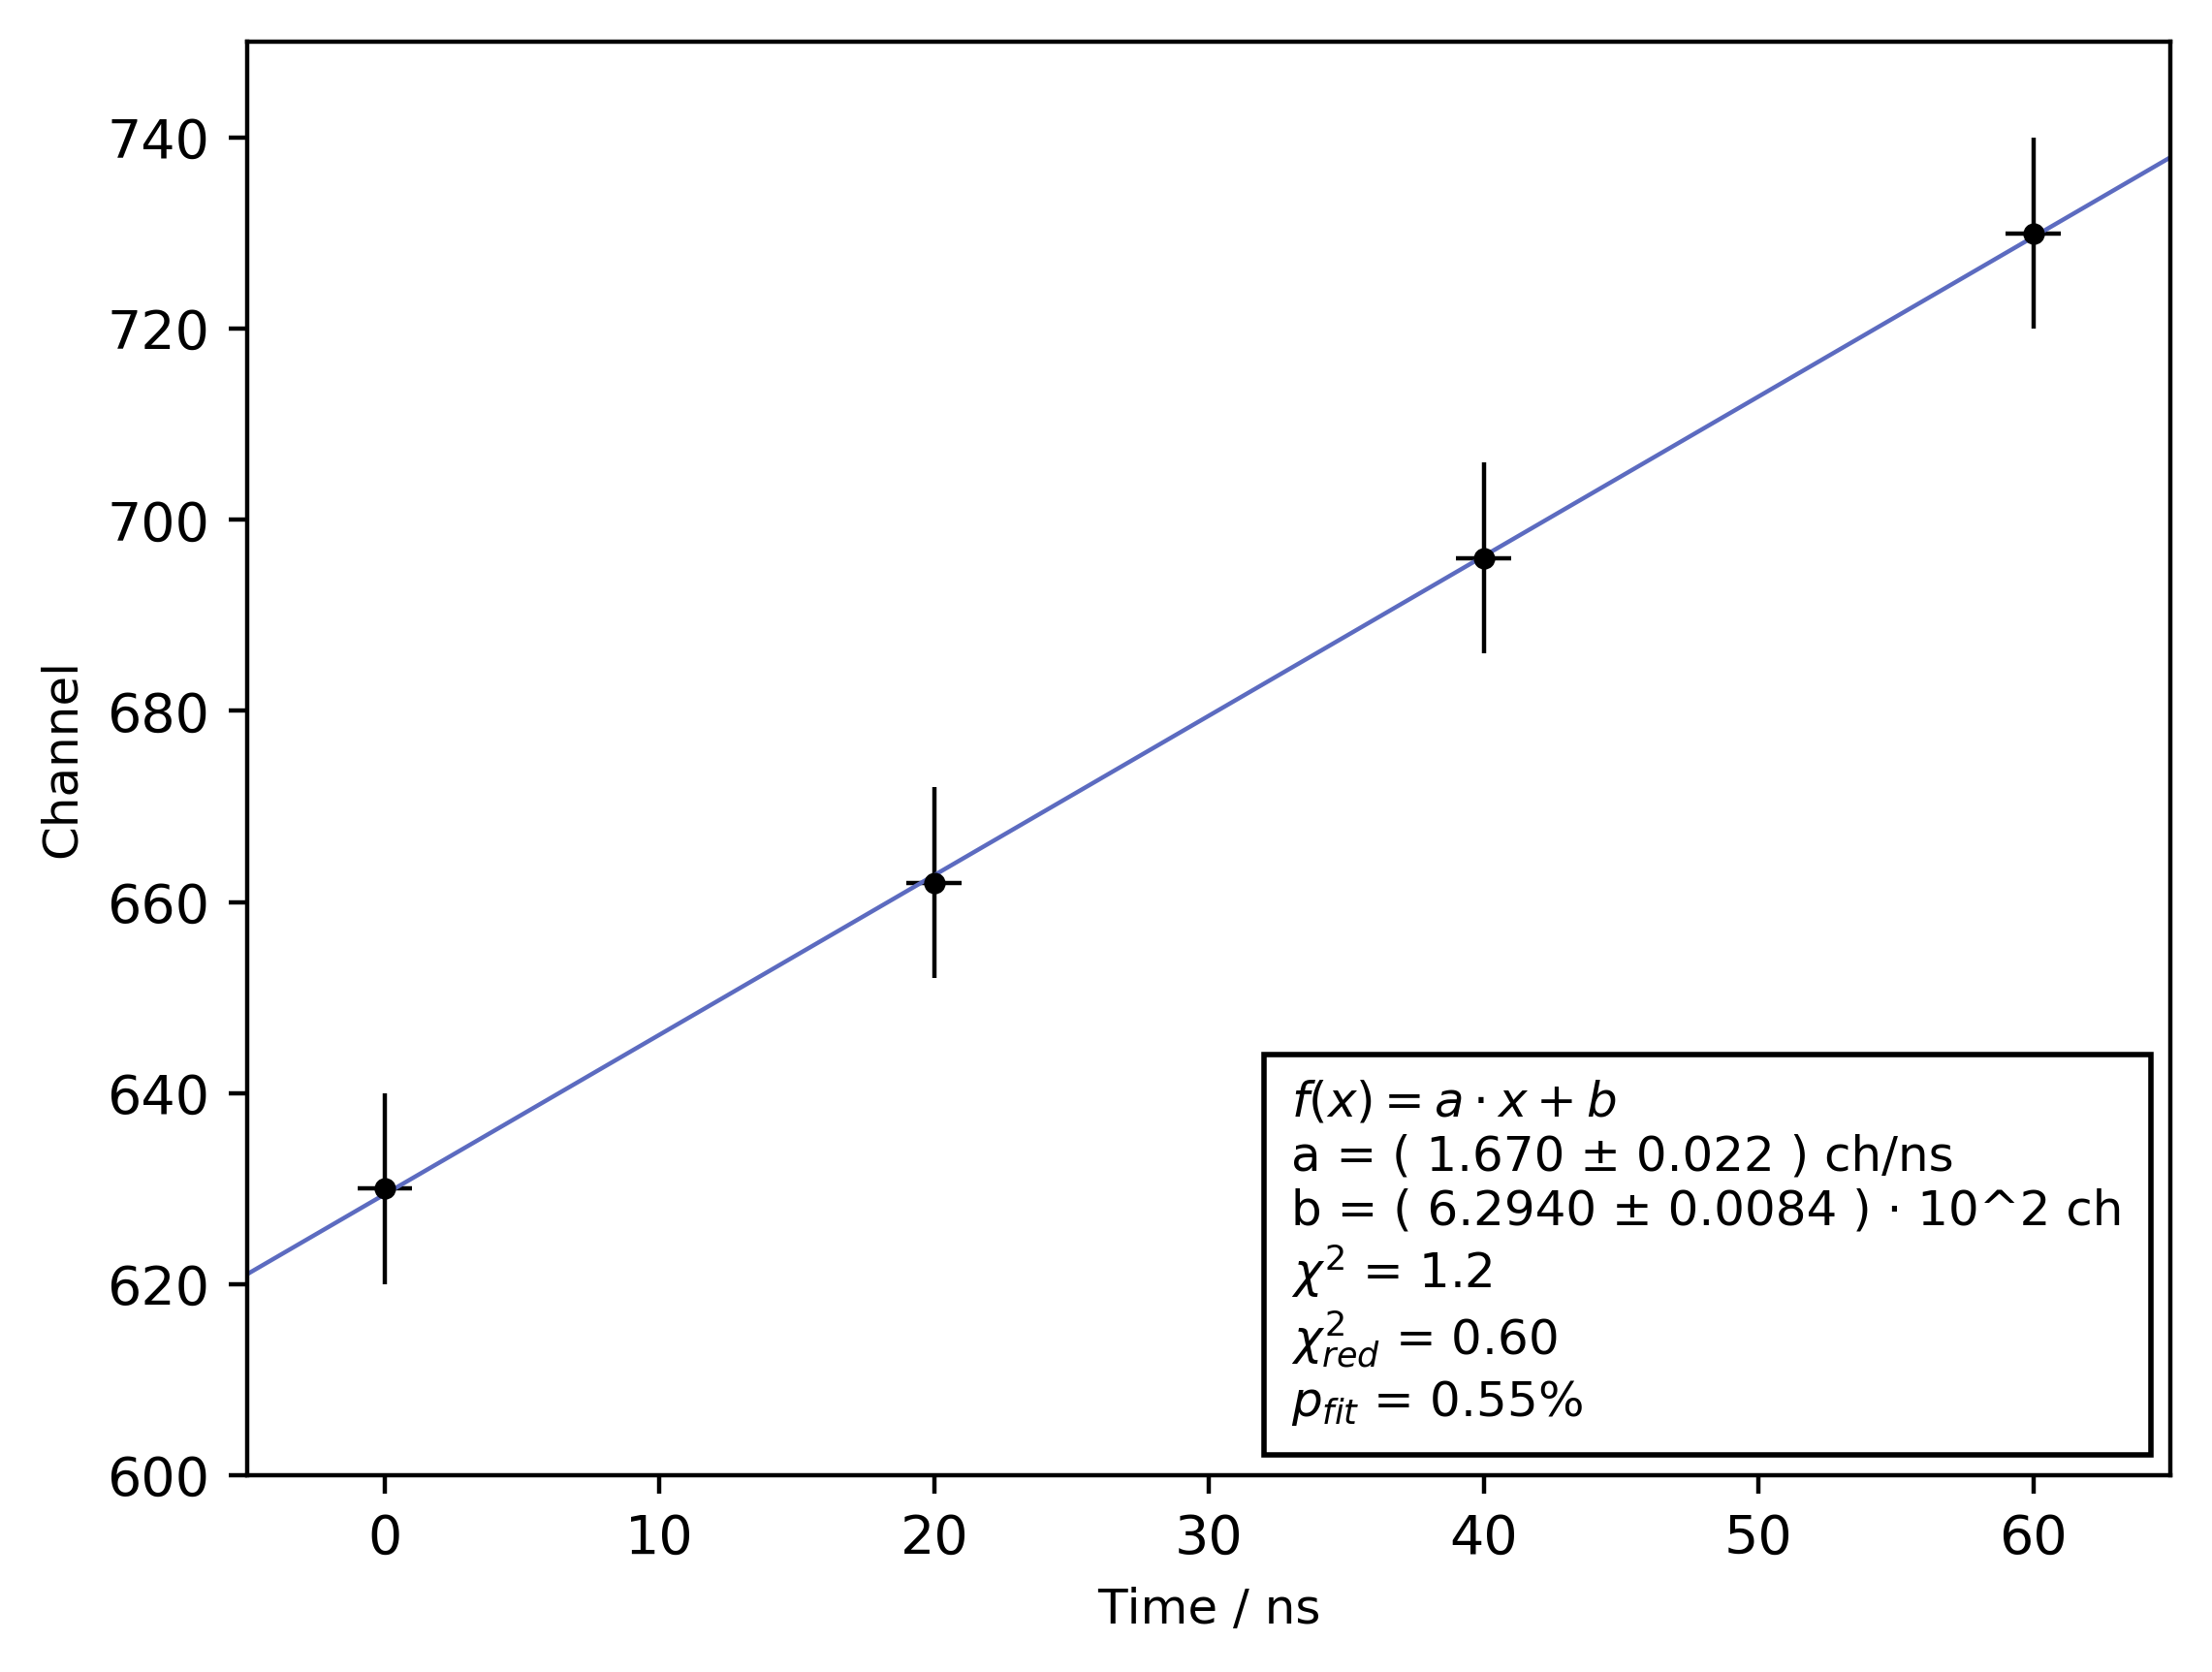
\includegraphics[]{png/time_calibration-cs}
        \end{adjustbox}
        \captionof{figure}{Time calibration for $^{137}\text{Cs}$ sample}
        \label{fig:TimeCalibrationCs}
    \end{center}
\endminipage
%
\par
%
\minipage{\linewidth}
    \begin{center}
        \captionsetup{type=figure}
        \begin{adjustbox}{max width=\linewidth, keepaspectratio}
            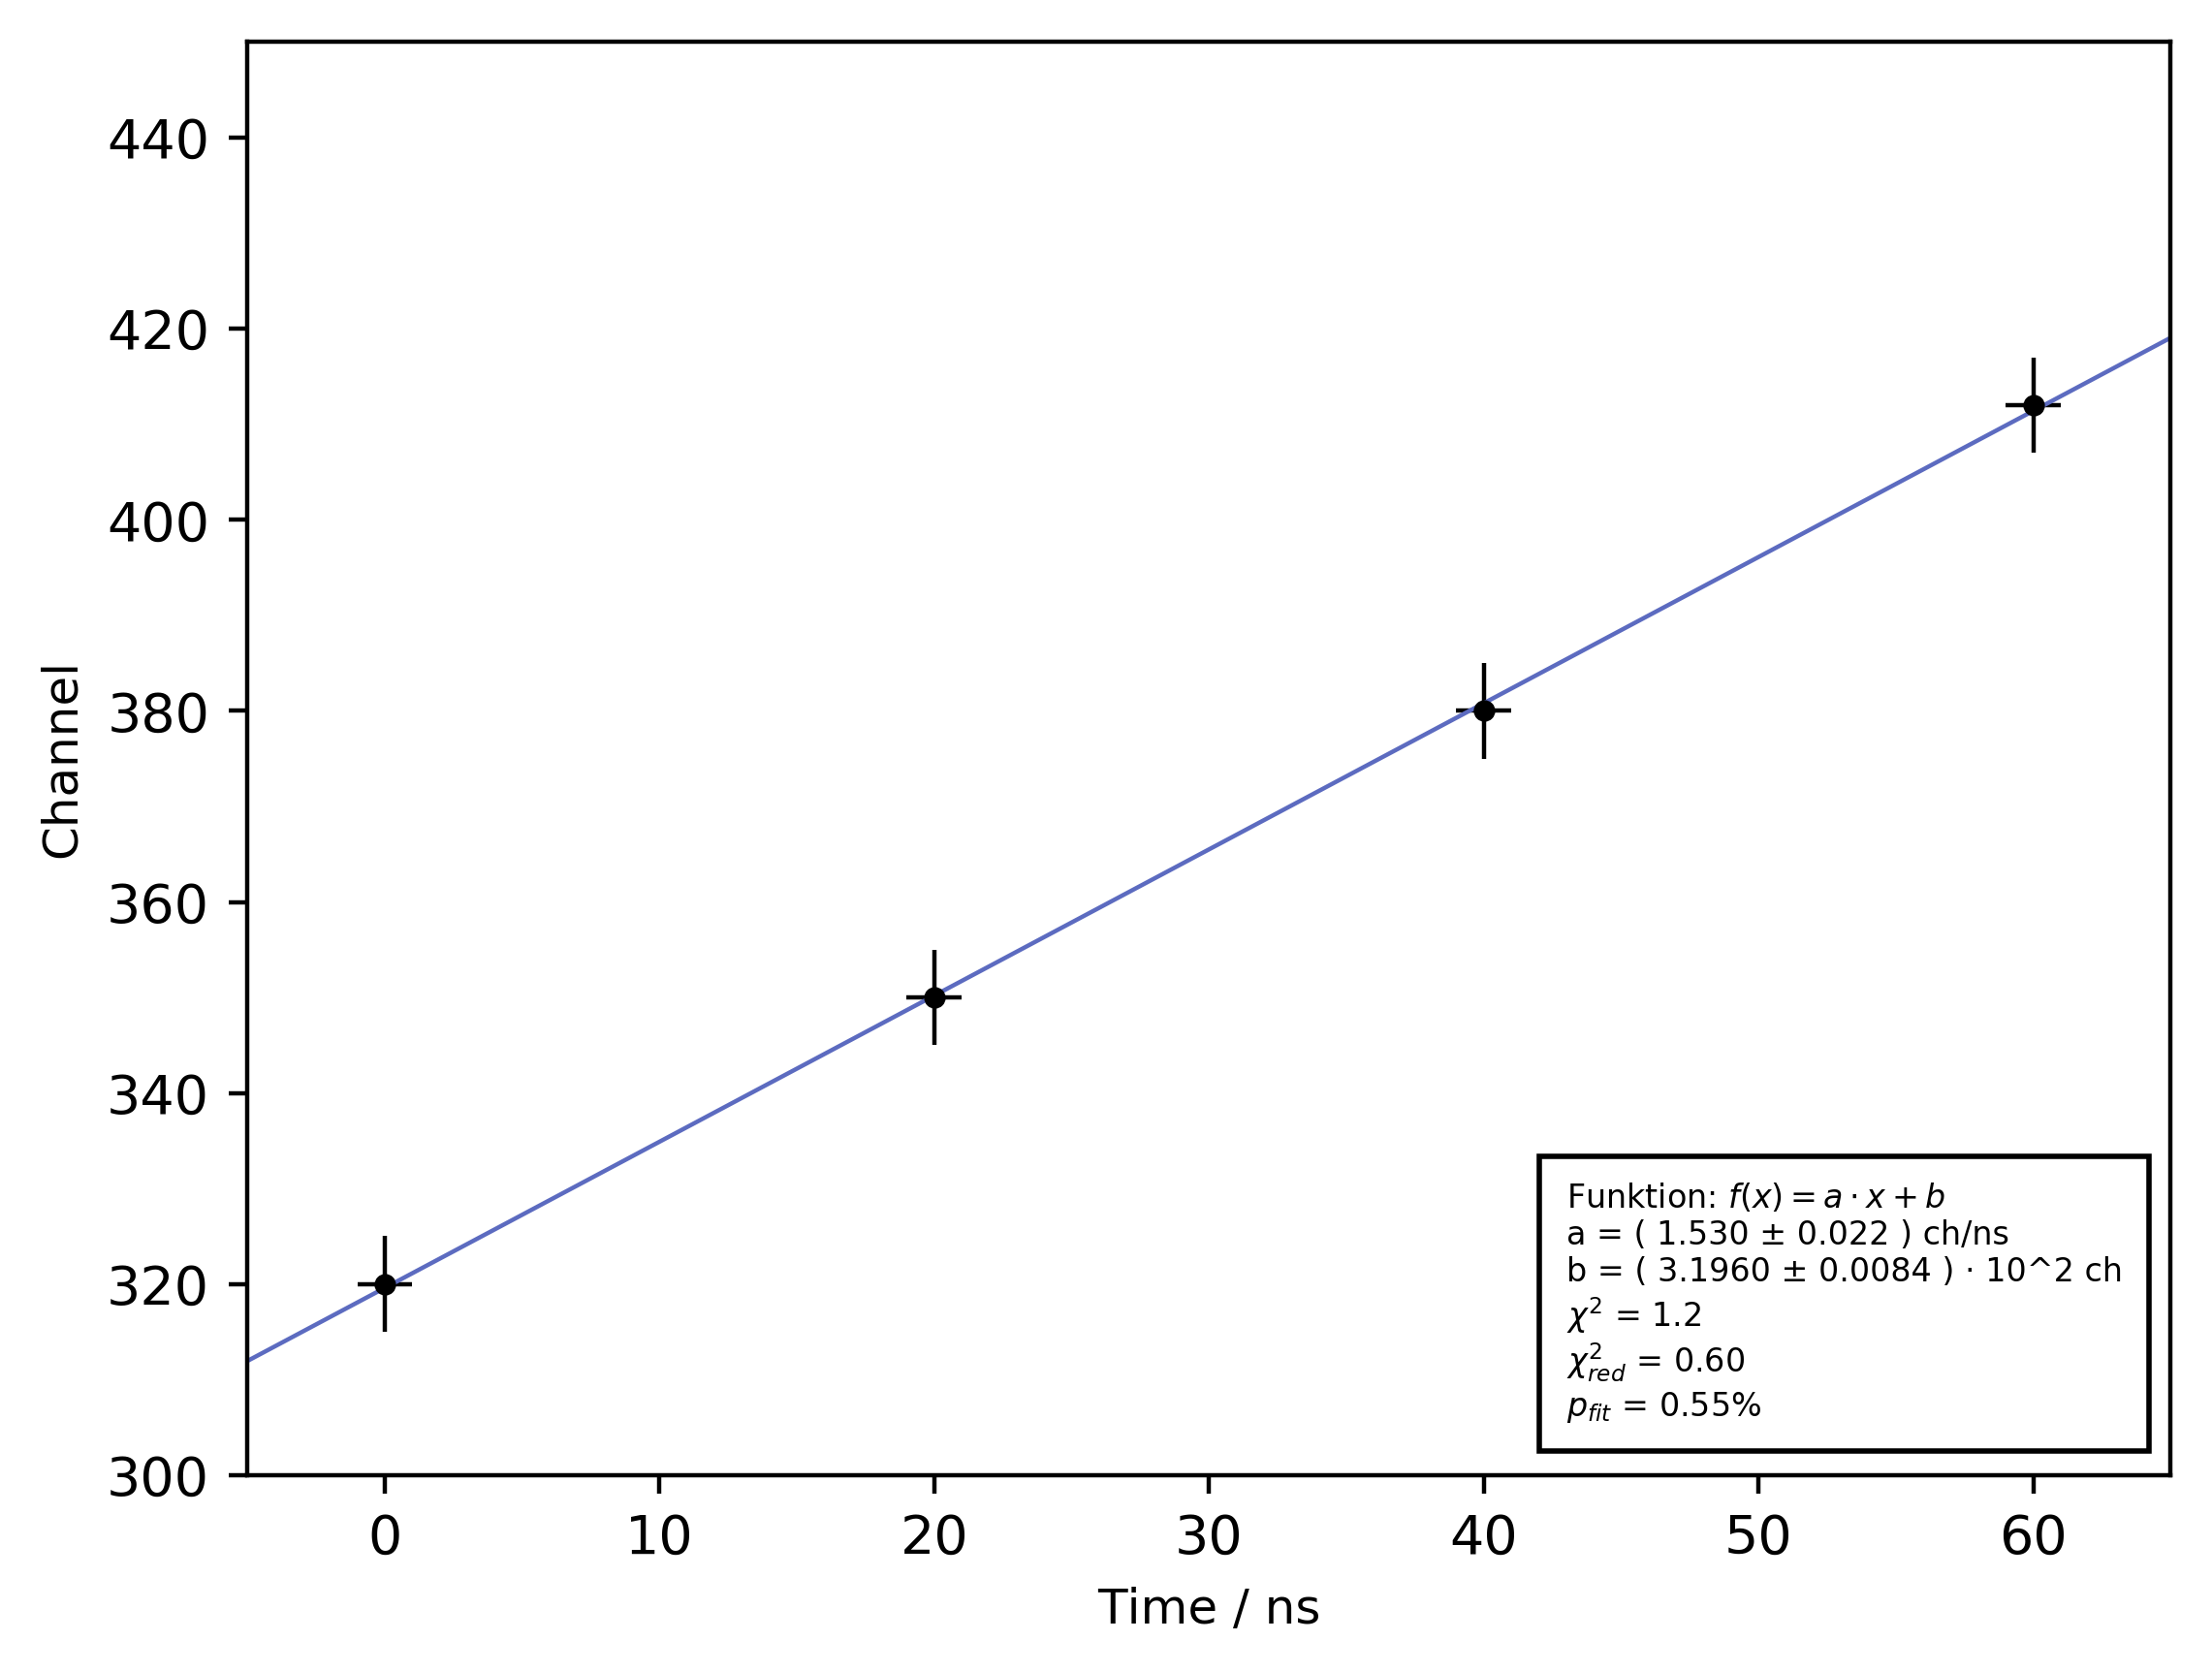
\includegraphics[]{png/time_calibration-co}
        \end{adjustbox}
        \captionof{figure}{Time calibration for $^{60}\text{Co}$ sample}
        \label{fig:TimeCalibrationCo}
    \end{center}
\endminipage
%
\par
%
Now, we are able to use the calibration to calculate the coincidence resolution $t$, which is defined by the width of the peak in the time spectrum.
Again, we use the FWHM:
%
\begin{align}
    \label{eq:CoincidenceResolution}
    \begin{split}
        t &= \frac{\xi _{\text{right}}- \xi _{\text{left}}}{a}
    \end{split}
    \\
    \label{eq:DeltaCoincidenceResolution}
    \begin{split}
        \Delta t &= \sqrt{ \left (  \frac{\xi _{\text{right}}- \xi _{\text{left}}}{a^2} \Delta a \right)^2 + 2 \left ( \frac{ \Delta \xi }{a}\right)^2 }
    \end{split}
\end{align}
%
Here we estimate $\Delta \xi = 3$.
We only use the first spectrum, because taking the mean of the four spectra would not decrease the systematic error significantly.
We obtain $t = \SI{59.9 \pm 2.7}{\nano\second}$.
%
\subsubsection{Time window}
%
For the spectrum as seen in figure \ref{fig:137CsmitTPHC_gated} we adjusted the time window at the Single Channel Analyzer.
Consequently, we managed to significantly reduce the height of the photo peak.
Additionally, the background noise of random coincidence is reduced while leaving the actual coincidental peaks untouched.
%
\subsubsection{Energy and time window}
%
Having blocked all signals from counter 2 that do not fall in the energy window of the backscatter peak, the spectrum now only shows the coincident Compton peak at its expected energy of $E_{\text{exp}} = \SI{0.46 \pm 0.04}{\mega\electronvolt}$.
The deviation to the theoretical value from above is not significant with 0.35 $\sigma$.
The random coincidence is highly suppressed.
%
\subsection{Coincidence measurement of $^{60}\text{Co}$ cascade decay}
%
The two photons of the $^{60}\text{Co}$ cascade decay can be considered simultaneous, because the life span of the intermediate state is only about \SI{0.7}{\pico\second}.
%
\subsubsection{Time resolution}
%
As with the $^{137}\text{Cs}$ measurements, we calibrate the time spectrum in figure \ref{fig:TimeCalibrationCo} and calculate the coincidence resolution to $t = \SI{ 13.1 \pm 2.8 }{\nano\second}$ using (\ref{eq:CoincidenceResolution}) and (\ref{eq:DeltaCoincidenceResolution}).
Because the peaks in the time spectrum are much more narrow, correspondingly, the time is shorter.
%
\subsubsection{Source strength and detection rates}
%
The detection rates $R$ of the scintillation detectors are given by:
%
\begin{align}
    \label{eq:DetectionRates}
    \begin{split}
        R_i &= M_i \cdot Q \cdot \eta_i ~~~~~ i \in \{1,2\}
    \end{split}
\end{align}
%
with the source strength $Q$, the detection probability of the detector $\eta_i$ and the photon multiplicity $M_i$ of the relevant radiation process.
In the same way the coincidence rate is given by:
%
\begin{align}
    \label{eq:CoincidenceDetectionRates}
    \begin{split}
        R_{\text{c}} &= M_{\text{c}} \cdot Q \cdot \eta_1 \cdot \eta_2
    \end{split}
\end{align}
%
While we do not know the detection probabilities, we can still combine the measured detection rates to calculate the source strength.
In our setup, coincident photons have two possibilities to be detected, so we use $M_{\text{c}} = 2$, while $M_1 = M_2 = 1$.
%
\begin{align}
    \label{eq:SourceStrength}
    \begin{split}
        Q &= \frac{R_1 R_2}{R_{\text{c}}} \frac{ M_{\text{c}}}{M_1 M_2} = 2 \frac{R_1 R_2}{R_{\text{c}}}
    \end{split}
\end{align}
%
The rates are calculated from the measured times $t_i$ and counts $N_i$ with
%
\begin{align}
    \label{eq:RateMeasured}
    \begin{split}
        R_i  &= \frac{N_i}{t_i}
    \end{split}
    \\
    \label{eq:DeltaRateMeasured}
    \begin{split}
        \Delta R_i &= \frac{\sqrt{N_i}}{t_i}
    \end{split}
\end{align}
%
with the statistical error for $N_i$.
This leads to an error in the source strength of:
%
\begin{align}
    \label{eq:DeltaSourceStrength}
    \begin{split}
        \Delta Q &= \sqrt{ \left ( \frac{\Delta R_1}{R_1} \right ) ^2 +
                           \left ( \frac{\Delta R_2}{R_2} \right ) ^2 +
                           \left ( \frac{\Delta R_{\text{c}}}{R_{\text{c}}} \right ) ^2 } \cdot Q
    \end{split}
\end{align}
%
The data is presented in table \ref{tab:DetectionRates}.
In total, we get a source strength of $Q = \SI{ 23.9 \pm 0.5 }{\kilo\becquerel}$.
%
\par
%
\minipage{\linewidth}
    \begin{center}
        \captionsetup{type=table}
        \begin{adjustbox}{max width=\linewidth, keepaspectratio}
            \begin{tabular}{llll}
            \toprule
            ~              & Time [\SI{}{\second}] & Counts           & Rate [\SI{}{\per\second}] \\
            \midrule
            $Q_1$          & 300                   & 87576 $\pm$ 300  & 291.9 $\pm$ 1.0           \\
            $Q_2$          & 317                   & 92712 $\pm$ 300  & 292.5 $\pm$ 1.0           \\
            $Q_{\text{c}}$ & 361                   & 2592 $\pm$ 51    & 7.18 $\pm$ 0.14           \\
            $Q_{\text{r}}$ & 361                   & 582 $\pm$ 24     & 1.61 $\pm$ 0.07           \\
            \bottomrule
            \end{tabular}
        \end{adjustbox}
        \captionof{table}{Experimental results of detection rates [TODO $Q_c$ und $Q_r$ erklären?]}
        \label{tab:DetectionRates}
    \end{center}
\endminipage
%
\par
%
The theoretical value $Q_{\text{theo}}$ can be calculated from the half life $t_{\nicefrac{1}{2}}$ of the isotope and the noted source strength $Q_0$ at a time $t$ before the experiment:
%
\begin{align}
    \label{eq:TheoSourceStrength}
    \begin{split}
        Q_{\text{theo}} &= Q_0 \cdot \exp(-\ln(2) \frac{t}{t_{\nicefrac{1}{2}}})
    \end{split}
    \\
    \label{eq:DeltaTheoSourceStrength}
    \begin{split}
        \Delta Q_{\text{theo}} &= \frac{ \Delta Q_0 }{ Q_0 } \cdot Q_{\text{theo}}
    \end{split}
\end{align}
%
\par
%
This gives $Q_{\text{theo}} = \SI{80.4 \pm 2.4}{\kilo\becquerel}$.
The high deviation of \SI{23}{\sigma} will be discussed later.
%
\par
%
Now, we can use the source strength to calculate the detection probabilities and compare them:
% 
\begin{align}
    \label{eq:DetectionProb}
    \begin{split}
        \eta_i &= \frac{ R_i }{ Q }
    \end{split}
    \\
    \label{eq:DeltaDetectionProb}
    \begin{split}
        \Delta \eta_i &= \sqrt{ \left ( \frac{ \Delta R_i }{ R_i } \right ) ^2 +
                                \left ( \frac{ \Delta Q }{ Q } \right ) ^2 } \cdot \eta_i
    \end{split}
\end{align}
%
This yields $\eta_1 = \SI{1.227 \pm 0.025}{\percent}$ and $\eta_2 = \SI{1.230 \pm 0.025}{\percent}$.
%
\subsubsection{Random coincidence}
%
From the measurement of the coincidence rate as seen in figure \ref{fig:60CoZeitspektrum}, we can extract the rate of random coincidence by counting the number of data not in the maximum and using equation (\ref{eq:RateMeasured}).
The result is also presented in table \ref{tab:DetectionRates}.
Again, the error is the statistical error given by $\sqrt{N_{\text{r}}}$.
The theoretical value can be obtained with
%
\begin{align}
    \label{eq:RandomCoincidence}
    \begin{split}
        R_{\text{r}}^{\text{theo}} &= 2 \cdot R_1 \cdot R_2 \cdot t_{\text{c}}
    \end{split}
    \\
    \label{eq:DeltaRandomCoincidence}
    \begin{split}
        \Delta R_{\text{r}}^{\text{theo}} &= \sqrt{ \left ( \frac{\Delta R_1}{R_1} \right ) ^2 +
                            \left ( \frac{\Delta R_2}{R_2} \right ) ^2 } \cdot R_{\text{r}}^{\text{theo}}
    \end{split}
\end{align}
%
where $t_{\text{c}}$ is the time frame for coincidence depicted by the circuit.
Because the SCA window was fully open, this means $t = \SI{2}{\micro\second}$ in our case.
This results in $R_{\text{r}}^{\text{theo}} = \SI{3.415 \pm 0.016 e-1}{\per\second}$.
The deviation of the values is \SI{19}{\sigma}.
%
\subsubsection{Qualitative observation of coincidence}
%
When we only allow simultaneous photons with an energy of one of the peaks to trigger the detection, we accordingly only detect photons of the other one.
Thus proving the coincident relationship.
%
